\section{实验结果与数据分析}

实验部分围绕三个问题展开。第一，NPQR 在代表性线路上是否能生成通过复放的路由
结果。第二，在同一线路和同一拓扑下，NPQR 相比 SABRE basic 能减少多少 SWAP。
第三，初始映射、束搜索、模型评分和局部修复这些设计在运行成本和结果质量上分别
起到什么作用。

\subsection{实验设置}

主实验采用固定对照口径。20 比特以内线路使用 Tokyo 20Q 拓扑，30/50 比特扩展线路
使用规则网格拓扑；NPQR 与 SABRE basic 使用相同输入线路、相同拓扑和相同指标字段。
SABRE basic 作为固定基线，只用于质量比较；NPQR 路线由自研流程生成，并经过轨迹
复放后进入表格。

\begin{table}[H]
  \centering
  \caption{实验指标说明}
  \label{tab:metrics}
  \begin{tabularx}{\linewidth}{lYY}
    \toprule
    指标 & 含义 & 解释方式 \\
    \midrule
    完成状态 & 是否成功生成满足约束的路由结果 & 是底线指标，未完成时 SWAP 和深度比较意义有限。 \\
    SWAP 数 & 插入的交换门数量 & 越低通常表示路由额外开销越小。 \\
    电路深度 & 路由后门序列的层数 & 越低通常表示潜在执行时间和噪声暴露越少。 \\
    运行时间 & 编译请求耗时 & 越低越适合在线接口和课堂演示。 \\
    轨迹复放 & 按输出轨迹重新验证拓扑合法性 & 用于确认结果不是仅由启发式分数推断。 \\
    基线差异 & 与 SABRE 指标的对照 & 用于观察算法表现边界，不作为唯一成功标准。 \\
    \bottomrule
  \end{tabularx}
\end{table}


实验指标见表 \ref{tab:metrics}。完成状态是先决指标：只有所有原始门被执行、每个
双比特门都满足硬件边约束、轨迹可以从初始映射复放到最终映射时，结果才记为完成。
在完成前提下，SWAP 数衡量额外交换开销，线路深度衡量可并行执行层数，运行时间衡量
在线演示和批量复现实验的计算成本。

\subsection{基础实验}

10/20 比特实验是本报告的主要质量证据。样例覆盖 GHZ、QFT、QAOA、VQE、随机线路
和结构化 20 比特线路，分别对应链式纠缠、长程交互、局部哈密顿量结构、变分线路和
较不规则的双比特门分布。

\begin{table}[H]
  \centering
  \caption{10/20 比特代表电路与 SABRE basic 的最终对比}
  \label{tab:final-basic-matrix}
  \begin{tabular}{lrrrr}
    \toprule
    电路 & 比特数 & NPQR SWAP & SABRE basic SWAP & 差值 \\
    \midrule
    GHZ10 & 10 & 2 & 6 & -4 \\
    QFT10 & 10 & 6 & 13 & -7 \\
    QAOA10 & 10 & 0 & 15 & -15 \\
    VQE10 & 10 & 1 & 4 & -3 \\
    Random10 & 10 & 17 & 19 & -2 \\
    Brickwork20 & 20 & 15 & 31 & -16 \\
    CliqueBlocks20 & 20 & 19 & 38 & -19 \\
    DeepRandom20 & 20 & 105 & 135 & -30 \\
    RingEntangler20 & 20 & 16 & 41 & -25 \\
    SparseRandom20 & 20 & 37 & 57 & -20 \\
    \bottomrule
  \end{tabular}
\end{table}


表 \ref{tab:final-basic-matrix} 显示，NPQR 在 10 个代表样例上全部完成路由，SWAP
数均低于 SABRE basic。10 个样例合计，NPQR 插入 218 个 SWAP，SABRE basic 插入
359 个，减少 141 个，降幅为 39.3\%。其中 10 比特样例从 57 个降至 26 个，20 比特
样例从 302 个降至 192 个。

图 \ref{fig:swap-comparison} 选取不超过 70 个 SWAP 的代表行画成柱状图，避免
DeepRandom20 这类大值压缩其他样例的视觉差异。结构化线路的收益最明显：QAOA10
从 15 个 SWAP 降至 0 个，CliqueBlocks20 从 38 个降至 19 个，RingEntangler20 从
41 个降至 16 个。随机线路的改善幅度相对小一些，但仍保持同向：Random10 减少
2 个 SWAP，SparseRandom20 减少 20 个 SWAP。这说明 NPQR 的收益并不只来自某一个
特定样例，而是同时出现在结构化线路和随机线路中。

\begin{figure}[H]
  \centering
  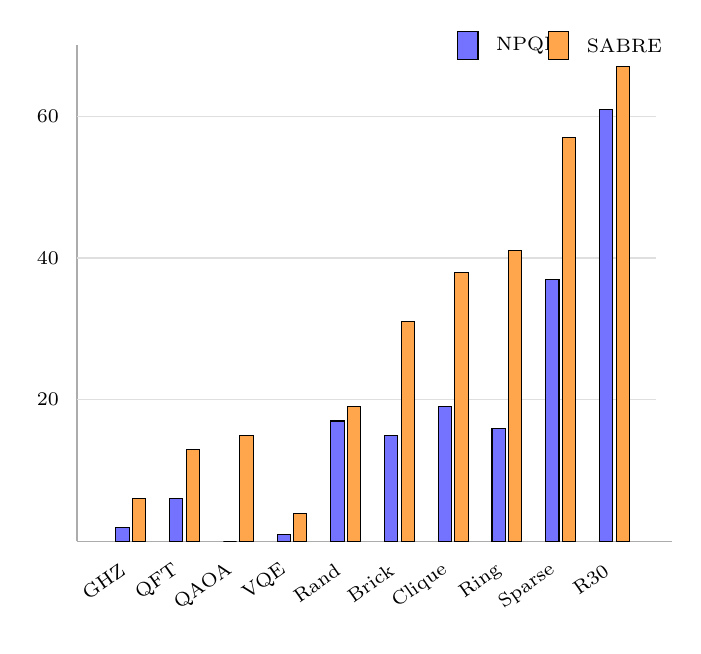
\begin{tikzpicture}[
  x=1.05cm,
  y=0.09cm,
  font=\scriptsize,
  axis/.style={draw=gray!65},
  npqr/.style={fill=blue!55},
  sabre/.style={fill=orange!70}
]
  \draw[axis] (0,0) -- (7.2,0);
  \draw[axis] (0,0) -- (0,70);
  \foreach \y in {20,40,60} {
    \draw[gray!25] (0,\y) -- (7.0,\y);
    \node[anchor=east] at (-0.1,\y) {\y};
  }

  \def\npqrvals{2,6,0,1,17,15,19,16,37,61}
  \def\sabrevals{6,13,15,4,19,31,38,41,57,67}
  \foreach \n [count=\i from 1] in \npqrvals {
    \pgfmathsetmacro{\x}{0.65*\i}
    \draw[npqr] (\x-0.18,0) rectangle (\x-0.02,\n);
  }
  \foreach \s [count=\i from 1] in \sabrevals {
    \pgfmathsetmacro{\x}{0.65*\i}
    \draw[sabre] (\x+0.02,0) rectangle (\x+0.18,\s);
  }

  \foreach \label [count=\i from 1] in {GHZ,QFT,QAOA,VQE,Rand,Brick,Clique,Ring,Sparse,R30} {
    \pgfmathsetmacro{\x}{0.65*\i}
    \node[rotate=35, anchor=east] at (\x,-3) {\label};
  }
  \draw[npqr] (4.6,68) rectangle (4.85,72);
  \node[anchor=west] at (4.95,70) {NPQR};
  \draw[sabre] (5.7,68) rectangle (5.95,72);
  \node[anchor=west] at (6.05,70) {SABRE};
\end{tikzpicture}

  \caption{SWAP 对比}
  \label{fig:swap-comparison}
\end{figure}

\subsection{拓展实验}

扩展实验选择 30/50 比特网格样例，用来观察同一套路由流程在更大拓扑上的表现。这里
不把扩展样例作为全规模能力结论，而是作为补充实验：线路规模增大后，初始映射和搜索
仍需在受限耦合图上给出可复放路线。

\begin{table}[H]
  \centering
  \caption{扩展实验}
  \label{tab:scale-smoke}
  \begin{tabular}{lrrrr}
    \toprule
    线路 & 比特数 & NPQR SWAP & SABRE basic SWAP & 差值 \\
    \midrule
    LineGHZ30 & 30 & 23 & 43 & -20 \\
    Random30-d4 & 30 & 61 & 67 & -6 \\
    LineGHZ50 & 50 & 50 & 79 & -29 \\
    RingSparse50 & 50 & 98 & 113 & -15 \\
    \bottomrule
  \end{tabular}
\end{table}


表 \ref{tab:scale-smoke} 中 4 个扩展样例全部完成，且 SWAP 数均低于 SABRE basic。
LineGHZ30 从 43 个 SWAP 降至 23 个，LineGHZ50 从 79 个降至 50 个；这类链式纠缠
线路受益于较好的初始布局。Random30-d4 和 RingSparse50 的改善幅度较小，分别减少
6 个和 15 个 SWAP，说明在较不规则交互下，NPQR 仍能形成优势，但搜索压力更高。

\subsection{消融实验}

消融实验采用 10 比特子集，固定 Tokyo 20Q 拓扑和相同最大步数，只改变路由组件。
该组实验用于观察模块作用，不替代主实验结论。完整配置包含结构化初始映射、多候选
束搜索和模型动作评分；单步选择把束宽和分支数都降为 1；简单映射减少初始映射候选
和局部布局优化。

\begin{table}[H]
  \centering
  \caption{消融实验}
  \label{tab:ablation-study}
  \begin{tabularx}{\linewidth}{lrrY}
    \toprule
    配置 & 完成数 & 完成样例 SWAP 合计 & 观察 \\
    \midrule
    完整配置 & 4/4 & 23 & GHZ10、QFT10、QAOA10、VQE10 全部完成。\\
    单步选择 & 1/4 & 0 & 只完成 QAOA10，长程交互样例容易停滞。\\
    简单映射 & 2/4 & 22 & QFT10 和 QAOA10 完成，但 QAOA10 需要额外 SWAP。\\
    \bottomrule
  \end{tabularx}
\end{table}


表 \ref{tab:ablation-study} 显示，完整配置在 4 个样例上全部完成。去掉多候选保留后，
只有 QAOA10 完成；GHZ10、QFT10 和 VQE10 都在有限步数内停住。弱化初始映射后，
完成数提高到 2 个，但 GHZ10 和 VQE10 仍未完成，QAOA10 的 SWAP 数也从 0 增加到
3。这个结果支持方法章节中的判断：束搜索负责避免过早陷入局部路线，结构化映射负责
降低搜索起点的距离代价。

模型评分另做了动作价值信号分析。对 15 组正负路线状态，模型在 12 组中给可取路线
更高分，正向比例为 80\%，平均分差为 0.00213。这个数值不直接等同于 SWAP 降幅，
但说明模型评分具有可用于排序的局部信号；最终路线质量仍由动作掩码、束搜索、修复
和复放共同决定。

\subsection{运行过程}

为了解释运行成本，项目对 NPQR 主流程做了分阶段计时。计时覆盖预处理、依赖关系、
拓扑距离矩阵、逻辑交互图、初始映射候选、主搜索、动作生成、模型推理、束搜索
剪枝、后处理、局部修复和轨迹复放。表 \ref{tab:phase-timing} 选取三个代表样例：
QAOA10、QFT10 和 Brickwork20。

\begin{table}[H]
  \centering
  \caption{阶段耗时}
  \label{tab:phase-timing}
  \begin{tabularx}{\linewidth}{lrlrY}
    \toprule
    样例 & 规模 & 总耗时 & 最耗时阶段 & 搜索子阶段观察 \\
    \midrule
    QAOA10 & 10Q & $623.9\mathrm{ms}\pm61.2\mathrm{ms}$ &
    初始映射候选生成 92.6\% & 结构化线路主要由初始映射吸收路由成本。\\
    QFT10 & 10Q & $16.23\mathrm{s}\pm1.14\mathrm{s}$ &
    主搜索阶段 90.2\% & 模型推理约 7.75s，束搜索扩展与剪枝约 5.65s。\\
    Brickwork20 & 20Q & $13.35\mathrm{s}\pm0.86\mathrm{s}$ &
    初始映射候选生成 99.8\% & 20Q 候选映射成为主要成本。\\
    \bottomrule
  \end{tabularx}
\end{table}

图 \ref{fig:timing-distribution} 展示三类样例的瓶颈差异。QAOA10 和 Brickwork20 的
耗时集中在初始映射候选生成，说明结构化交互线路的主要成本在起点选择；QFT10 的主
搜索占 90.2\%，其中模型推理和束搜索扩展是主要子项。这个结果与复杂度分析一致：
当线路包含更多长程依赖时，候选状态数量和动作评分次数会成为主要增长项。

\begin{figure}[H]
  \centering
  \begin{tikzpicture}[
  x=1.6cm,
  y=0.055cm,
  font=\scriptsize,
  axis/.style={draw=gray!65},
  init/.style={fill=blue!55},
  search/.style={fill=orange!70},
  other/.style={fill=gray!35}
]
  \draw[axis] (0,0) -- (5.2,0);
  \draw[axis] (0,0) -- (0,105);
  \foreach \y in {25,50,75,100} {
    \draw[gray!25] (0,\y) -- (4.9,\y);
    \node[anchor=east] at (-0.08,\y) {\y\%};
  }

  \draw[init] (0.65,0) rectangle (1.05,92.6);
  \draw[search] (1.05,0) rectangle (1.45,4.0);
  \draw[other] (1.45,0) rectangle (1.85,3.4);
  \node[anchor=north] at (1.25,-3) {QAOA10};

  \draw[init] (2.15,0) rectangle (2.55,4.0);
  \draw[search] (2.55,0) rectangle (2.95,90.2);
  \draw[other] (2.95,0) rectangle (3.35,5.8);
  \node[anchor=north] at (2.75,-3) {QFT10};

  \draw[init] (3.65,0) rectangle (4.05,99.8);
  \draw[search] (4.05,0) rectangle (4.45,0.1);
  \draw[other] (4.45,0) rectangle (4.85,0.1);
  \node[anchor=north] at (4.25,-3) {Brick20};

  \draw[init] (1.05,106) rectangle (1.3,111);
  \node[anchor=west] at (1.38,108.5) {初始映射};
  \draw[search] (2.2,106) rectangle (2.45,111);
  \node[anchor=west] at (2.53,108.5) {主搜索};
  \draw[other] (3.15,106) rectangle (3.4,111);
  \node[anchor=west] at (3.48,108.5) {其他};
\end{tikzpicture}

  \caption{耗时分布}
  \label{fig:timing-distribution}
\end{figure}

实验总体说明，NPQR 的质量收益来自多个组件的组合，而不是单一技巧。初始映射减少
搜索起点的拓扑距离，束搜索保留多条候选路线，模型评分提供局部动作偏好，局部修复
处理尾部停滞，轨迹复放保证结果可验证。运行时间仍有优化空间，尤其是候选映射生成、
模型推理和束搜索扩展；这些开销也为后续批处理推理、候选剪枝和分层路由提供了明确
方向。
